\chapter{Project Management}
\label{chapter4}

This section describes how the project will be conducted throughout the project's development. Details on risks and problems that may arise as well as the contingency plan for them is outlined here.

\section{Methodology}
The methodology that will be used for this project is the Agile methodlogy. This methodlogy will be used for this project as following the agile methodlogy gives you a working product earlier in the building phase. Agile also requires a weekly standup to be held, this will keep the project on schedule, as during this standup meeting the week's progress on the project will be checked and evaluated.  
\newline
\par
As part of the project schedule, there are two prototypes that are demonstrated to the supervisor. These prototypes shows significant development progress and features implemented. The first prototype shows a working demo with simple randomly generated graphs on flat ground as well as virtual reality features implemented. The virtual reality features will be limited to head and motion controller tracking in the game world, interaction with objects and teleportation navigation around the world. The second prototype will include terrain generation and Towers of Hanoi logic with water flow based on them. Having these prototype schedules makes sure that at certain points in the development there is a working product with features to show.
\newline
\par
The tasks outline in the project schedule in section 4.2 are evenly distributed for each member in the group. This is to maximise the amount of development that can be done so whilst someone is working on task, the other can work on a different task. This also helps with working on the project at the same time to avoid conflicts in code and development as each member is working on a different area.
\clearpage
\section{Schedule}
\begin{figure}[H]
	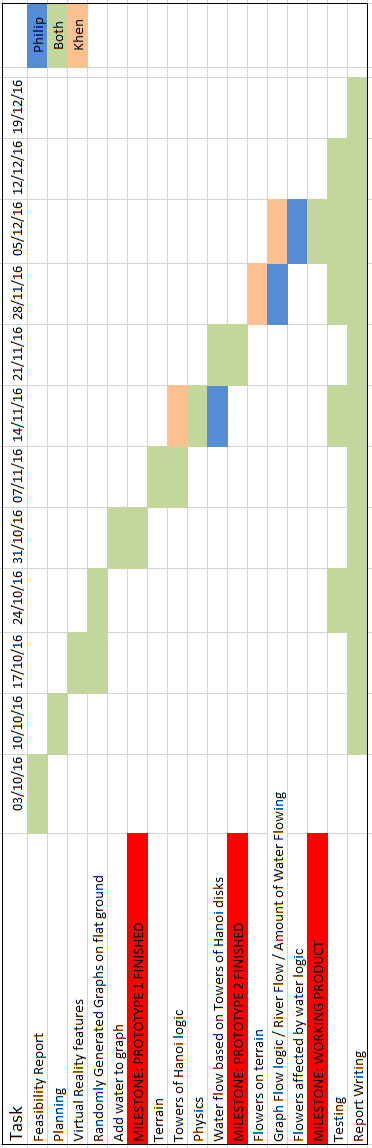
\includegraphics[height=23cm]{GanttChart}
	\centering
	\caption{Gantt Chart showing the work that will be done each week.}
	\label{fig:ganttChartPlan}
\end{figure}
\clearpage
\begin{tabular}{ |p{6cm}|p{3cm}| }
	\hline
	Writing Milestone & Date For
	\\\hline
	Layout Done & 14/11/2016
	\\\hline
	Chapter 1 - Introduction & 21/11/2016
	\\\hline
	Chapter 2 - Background & 28/11/2016
	\\\hline
	Chapter 3 - Requirements & 28/11/2016
	\\\hline
	Chapter 4 - Project Management & 05/12/2016
	\\\hline
	Chapter 5 - Planning and Design & 05/12/2016
	\\\hline
	Chapter 6 - Implementation & 12/12/2016
	\\\hline
	Chapter 7 - Testing and Evaluation & 12/12/2016
	\\\hline
	Chapter 8 - Conclusion & 12/12/2016
	\\\hline
	First Draft Complete & 12/12/2016
	\\\hline
	Report Finished & 23/12/2016
	\\\hline
\end{tabular}

\section{Version Control}
The Version control for this project will be done on GitHub. Version control software will be used for the project in order to accurately document any and all changes that will be made to the code. GitHub is the chosen version control service since it is the de facto standard for version control. Members are comfortable and familiar with using Git version control as opposed to others such as Mercurial.

\section{Risk Assessment}
A risk involved with this project is the availability of the HTC Vive headset as well as its peripherals. Since the tech demo will be making use of the Vive as the virtual reality hardware, it is essential that a Vive is at hand to be used for testing the demo. The school currently owns 2 Vive packages and since the school is currently only using them for demoing purposes of off the shelf demos and not for development, a Vive should be available for the development in this project. If there is no access to a HTC Vive headset, a contingency plan has been made, which is outlined in \ref{subsec:conPlan}.
\newline
\par
Another risk that may occur is that the Vive has certain requirements for the space it needs to use for a room-scale experience. The Vive takes some time to set up since it has to recalibrate to the environment every time it is set up again. This means a dedicated room where the Vive's base stations can be left set up is ideal. If a big enough room is not available, Vive has an option to use a standing/seated experience instead. This will means that user movement cannot be tested and movement in the virtual world will have to be restricted to Vive’s teleportation mechanic. The user looking around the world will still be supported with this version.
\newline
\par
One other factor that needs to be taken in to consideration is the availability of computer hardware that is powerful enough to run and develop on the HTC Vive. Since the HTC Vive has high minimum requirements to run it, finding a computer that is sufficient and can be used when needed can become an issue.

\subsection{Contingency Plan}\label{subsec:conPlan}
In the case that there is no access to a Vive headset for this project, due to the risks mentioned before, a contingency plan has been made. The plan would be to make a desktop application using the same premise, rather than being able to use the Vive for the game. This desktop application would have the same features as the Vive version, although without the VR features, i.e. looking around using the headset and interacting with objects using the controllers.
\newline
\par
The plan for dealing with if there is no room available is that a seated experience could be developed without need a room set-up. This would just involve setting up one camera above the computer and it would only track head movement. A standard game controller would have to be used for this set-up.
\newline
\par
For the risk that there is no high-end computer available, a high-end laptop that can run the software has already been acquired and will be used if there is no other computer available. The laptop is personally owned so there is no problem in accessibility.